\documentclass[12pt, border=8pt]{standalone}
\usepackage{tikz}
\usepackage{amsmath, amssymb, bm}
\usepackage{xcolor}
\usetikzlibrary{positioning, arrows.meta, calc, fit, backgrounds}

\begin{document}


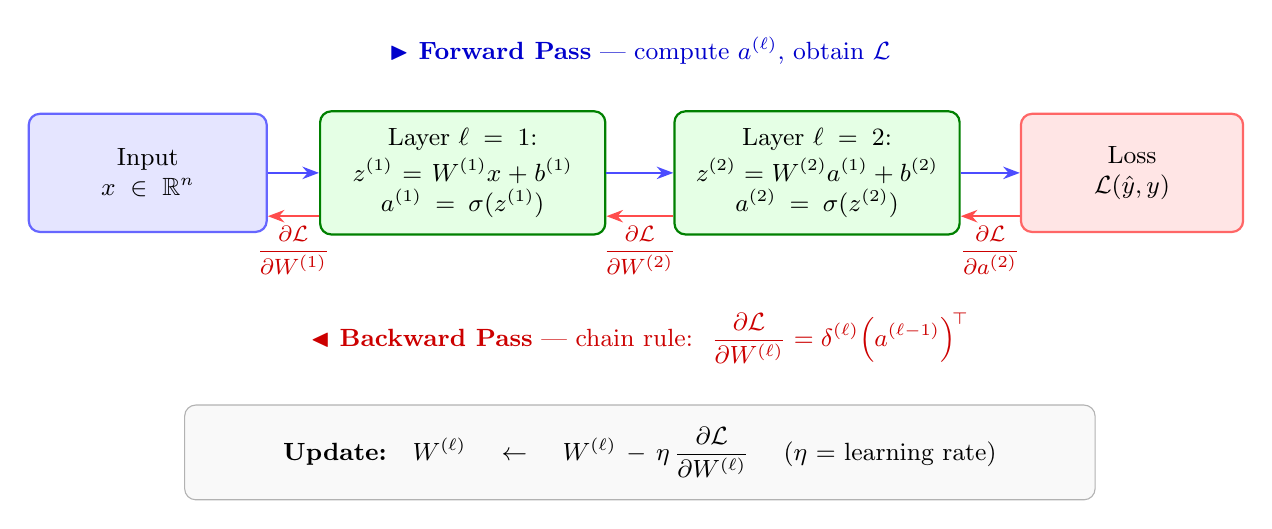
\begin{tikzpicture}[
  inputbox/.style={
    rectangle, draw=blue!60, fill=blue!10, thick,
    rounded corners=4pt, text width=2.6cm, align=center,
    minimum height=1.5cm, font=\small, inner sep=6pt
  },
  layerbox/.style={
    rectangle, draw=green!50!black, fill=green!10, thick,
    rounded corners=4pt, text width=3.2cm, align=center,
    minimum height=1.5cm, font=\small, inner sep=6pt
  },
  lossbox/.style={
    rectangle, draw=red!60, fill=red!10, thick,
    rounded corners=4pt, text width=2.4cm, align=center,
    minimum height=1.5cm, font=\small, inner sep=6pt
  },
  fwd/.style={-{Stealth[length=6pt]}, blue!70, thick},
  bwd/.style={-{Stealth[length=6pt]}, red!70, thick},
]

%% ── Pipeline boxes ───────────────────────────────────────────────────────────
\node[inputbox] (inp) at (0, 0) {Input\\$x \in \mathbb{R}^n$};

\node[layerbox] (l1) at (4.0, 0) {%
  Layer $\ell=1$:\\[2pt]
  $z^{(1)}=W^{(1)}x+b^{(1)}$\\
  $a^{(1)}=\sigma(z^{(1)})$
};

\node[layerbox] (l2) at (8.5, 0) {%
  Layer $\ell=2$:\\[2pt]
  $z^{(2)}=W^{(2)}a^{(1)}+b^{(2)}$\\
  $a^{(2)}=\sigma(z^{(2)})$
};

\node[lossbox] (loss) at (12.5, 0) {Loss\\$\mathcal{L}(\hat{y},y)$};

%% ── Forward arrows (top) ─────────────────────────────────────────────────────
\draw[fwd] (inp.east)  -- (l1.west);
\draw[fwd] (l1.east)   -- (l2.west);
\draw[fwd] (l2.east)   -- (loss.west);

\node[font=\small, blue!80!black] at (6.25, 1.55)
  {\textbf{$\blacktriangleright$ Forward Pass} --- compute $a^{(\ell)}$, obtain $\mathcal{L}$};

%% ── Backward arrows (bottom) ─────────────────────────────────────────────────
% loss → l2
\draw[bwd] ([yshift=-0.55cm]loss.west) -- ([yshift=-0.55cm]l2.east)
  node[midway, below, font=\footnotesize, red!80!black]
  {$\dfrac{\partial\mathcal{L}}{\partial a^{(2)}}$};

% l2 → l1
\draw[bwd] ([yshift=-0.55cm]l2.west) -- ([yshift=-0.55cm]l1.east)
  node[midway, below, font=\footnotesize, red!80!black]
  {$\dfrac{\partial\mathcal{L}}{\partial W^{(2)}}$};

% l1 → inp
\draw[bwd] ([yshift=-0.55cm]l1.west) -- ([yshift=-0.55cm]inp.east)
  node[midway, below, font=\footnotesize, red!80!black]
  {$\dfrac{\partial\mathcal{L}}{\partial W^{(1)}}$};

\node[font=\small, red!80!black] at (6.25, -2.1)
  {\textbf{$\blacktriangleleft$ Backward Pass} --- chain rule:\;
   $\dfrac{\partial\mathcal{L}}{\partial W^{(\ell)}}
    = \delta^{(\ell)}\!\left(a^{(\ell-1)}\right)^{\!\top}$};

%% ── Update rule box ──────────────────────────────────────────────────────────
\node[
  draw=gray!60, fill=gray!5, rounded corners=4pt,
  text width=11cm, align=center, font=\small,
  inner sep=8pt
] at (6.25, -3.55) {%
  \textbf{Update:}\quad
  $W^{(\ell)} \;\leftarrow\; W^{(\ell)} - \eta\,\dfrac{\partial\mathcal{L}}{\partial W^{(\ell)}}$
  \quad ($\eta$ = learning rate)
};

\end{tikzpicture}

\end{document}
